% This template was originally by R. Jacob Vogelstein
% Updated on March 1, 2010 by Noah J. Cowan


\documentclass[12pt,oneside,final]{thesis}
\usepackage{Sweave}
\usepackage{cite}
\usepackage{amsmath,amsfonts}
\usepackage{graphicx}
\graphicspath{{./figs/}}
\usepackage{fixltx2e}
\usepackage{array}
% wrapfig is fragile: use sparingly
\usepackage{wrapfig} 
%\usepackage{times}  % Use this for ugly fonts


\usepackage{fancyhdr}    % Use nice looking headers along with the required footer page numbers   
%\usepackage[hypertex]{hyperref}

%Define the header/footer style
\pagestyle{fancy}
\fancyhf{}
\setlength{\headheight}{15pt}
\lhead{\leftmark}
\cfoot{\thepage}
\renewcommand{\headrulewidth}{0pt}
\fancypagestyle{plain}{% Redefine ``plain'' style for chapter boundaries
\fancyhf{} % clear all header and footer fields
\fancyfoot[C]{\thepage} % except the center
\renewcommand{\headrulewidth}{0pt}
\renewcommand{\footrulewidth}{0pt}}

%\tolerance=10000

%\makeglossary % enable the glossary

\begin{document}
\input{thesis-concordance}

\title{JHU THESIS TEMPLATE}
\author{Sancar Adali}
\degreemonth{May}
\degreeyear{2007} 
\dissertation
\doctorphilosophy
\copyrightnotice


% add your chapters, best way is to have separate TeX files for each chapter
\input{chapter0}
\input{chapter1}
\input{chapter2}
\input{chapter3}
\input{chapter4}
\input{chapter5}
\input{chapter6}
\input{chapter7}
\input{chapter8}
\input{chapter9}
\input{chapter10}
\input{chapter11}

\include{appendix}

%% REFERENCES

% if you use BIBTEX
\bibliographystyle{IEEEtran}
\bibliography{thesis}

\begin{vita}

\begin{wrapfigure}{l}{0pt}
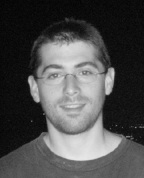
\includegraphics[width=2in,height=2.5in,clip,keepaspectratio]{rjvheadshot}
\end{wrapfigure}



\end{vita}
\end{document}
